\chapter{Graph-Theoretic Foundation}

The focus of this chapter will be \emph{multipartite graphs}, 
particularly \emph{bipartite graphs}, and their relationship 
to autosegmental morphology.
% which are a subset, i.e., special case, of multipartite graphs. 
A multipartite graph is a graph 
whose nodes can be partitioned into $N$ \emph{disjoint} sets of 
\emph{mutually nonadjacent} nodes, i.e., $N$ sets such that no two
nodes within the \emph{same} set are connected by an edge. A bipartite graph
is simply a multipartite graph where $N = 2$. That is, a graph is bipartite if it satisfies the following
criteria:
\begin{enumerate}
\item The graph's nodes are separated into two disjoint sets (or partitions).
\item Within each partition, all nodes are independent, i.e., mutually nonadjacent.
\end{enumerate}
Note that these two criteria are equivalent to the properties of nonlinearity and 
nonsequentiality, respectively, defined in section~\ref{sec:targets}.
Fig.~\ref{fig:bipartite} is a bipartite
graph; its nodes are divided into two partitions, the sets $M$
and $R$. Within each set, all nodes are independent; 
the only connections are between nodes of different sets.

In graph-theoretic terms, the multi-linear formalism of
\cite{mccarthy:1981} is a type of \emph{multipartite}
%, or $K$-partite, 
graph. This is a graph whose nodes can be partitioned into $N$ sets of
\emph{mutually nonadjacent} nodes, i.e., $N$ sets such that no two
nodes within the \emph{same} set are connected by an edge. %---% 
Fig.~\ref{fig:bipartite}, for example, shows a \emph{bipartite}
graph, i.e., a graph with two partitions, in this case the sets $M$
and $R$.
Within each set, all nodes are independent; the only connections are between nodes of different sets.

 \begin{figure}[htb]
 \begin{center}
 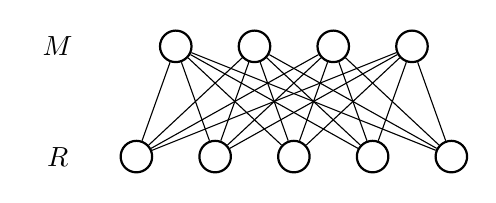
\begin{tikzpicture}[draw=black!100,scale=1.0]
 	\def \rowtwoht{1.4cm}
 	\def \rowoneht{0.0cm}
 	\tikzstyle{m-node}=[circle,draw=black!100,thick,inner sep=0pt,minimum size=4mm]
 	\tikzstyle{r-node}=[circle,draw=black!100,thick,inner sep=0pt,minimum size=4mm]
 	\tikzstyle{annot} = [text width=1.5em, text centered]
 	\node[annot] (hidden-label) at (-0.5cm,\rowtwoht) {$M$};
 	\node[annot] (surface-label) at (-0.5cm,\rowoneht) {$R$};
 	\node[m-node] 	(m0)	at (1cm,\rowtwoht)		{};
 	\node[m-node] 	(m1)	at (2cm,\rowtwoht)		{};
 	\node[m-node] 	(m2)	at (3cm,\rowtwoht)	 	{};
 	\node[m-node] 	(m3)	at (4cm,\rowtwoht) 		{};
 	% surface layer
 	\node[r-node] 	(r0)	at (0.5cm,\rowoneht)		{};
 	\node[r-node] 	(r1)	at (1.5cm,\rowoneht)		{};
 	\node[r-node] 	(r2)	at (2.5cm,\rowoneht)	 	{};
 	\node[r-node] 	(r3)	at (3.5cm,\rowoneht) 		{};
 	\node[r-node] 	(r4) 	at (4.5cm,\rowoneht)   		{};
 	%\node[r-node] 	(r5) 	at (6.5cm,\rowoneht)   		{};
 	\path (r0)	edge	node	{}	(m0)
		(r0)	edge	node	{}	(m1)
		(r0)	edge	node	{}	(m2)
		(r0)	edge	node	{}	(m3)

		(r1)	edge	node	{}	(m0)
		(r1)	edge	node	{}	(m1)
		(r1)	edge	node	{}	(m2)
		(r1)	edge	node	{}	(m3)

		(r2)	edge	node	{}	(m0)
		(r2)	edge	node	{}	(m1)
		(r2)	edge	node	{}	(m2)
		(r2)	edge	node	{}	(m3)
						
		(r3)	edge	node	{}	(m0)
		(r3)	edge	node	{}	(m1)
		(r3)	edge	node	{}	(m2)
		(r3)	edge	node	{}	(m3)

		(r4)	edge	node	{}	(m0)
		(r4)	edge	node	{}	(m1)
		(r4)	edge	node	{}	(m2)
		(r4)	edge	node	{}	(m3);
 		%(m3)	edge	node	{}	(r5);		
 \end{tikzpicture}
 \end{center}
 \caption{Bipartite graph}
 %. Neither layer contains sequential dependencies; every unit is independent within its own layer. Each hidden unit is thus free to cause any combination of observed units.}
 \label{fig:bipartite}
 \end{figure}


%Now, an MCMM, as it turns out, is a special case of a bipartite graph. Indeed,
%fig.~\ref{fig:bipartite} could itself be a simple MCMM. %precisely the architecture of an MCMM.
%%To sum up, bipartite graphs possess the properties nonlinerarity and nonsequentiality. 
%Because MCMMs are bipartite graphs, and bipartite graphs are both nonlinear and nonsequential, 
%MCMMs must themselves be nonlinear and nonsequential, which makes MCMMs well-suited for modeling
%non-concatenative morphology.

As it turns out, a bipartite graph suffices
%we do not need many partitions 
to capture the essential properties of McCarthy's autosegmental
framework,
% (fig.~\ref{subfig:nonlinear}). 
for a bipartite graph meets the two criteria stated in
(\ref{ex:criteria}).  We can reformulate the morpheme tiers and the
segmental tier in fig.~\ref{subfig:nonlinear} as the sets $M$ and
$R$, respectively, in fig.~\ref{fig:bipartite}---disjoint
by the definition of \emph{bipartite}. This satisfies the first
criterion. For the second, each node in $M$ represents a morpheme (or
morpheme tier), and, by the definition of \emph{bipartite}, the nodes
within $M$ are independent and thus orthogonal.

An MCMM (section~\ref{sec:mcmm}) is well-suited for the learning of
non-concatenative morphology because it is bipartite graph. It has two
\emph{layers} (equivalently, sets) of nodes, a hidden layer and a
surface layer---corresponding, respectively, to $M$ and $R$ in
fig.~\ref{fig:bipartite}. There are no intra-layer connections in an
MCMM, only connections between layers.
%, as in any bipartite graph.

We will henceforth refer to an MCMM's two partitions of nodes as
\emph{vectors} of nodes and will use matrix and vector notation to
describe the components of an MCMM:
%. That is, we will use
uppercase boldface letters refer to matrices, %(e.g., $\mathbf{M}$),
lowercase boldface letters refer to vectors,
% and matrix rows or columns, 
%(e.g., $\mathbf{m}_i$),
and italicized lowercase letters refer to the individual elements
of vectors/matrices. % (e.g., $m_{ik}$).
For example, $m_{i,k}$ is the $k^{\text{th}}$ element in the vector
$\mathbf{m}_i$, which is the $i^{\text{th}}$ row in the $I \times K$ matrix
$\mathbf{M}$. Thus, we will henceforth write the $M$ and $R$ in
fig.~\ref{fig:bipartite} as $\mathbf{m}$ and $\mathbf{r}$,
respectively (or $\mathbf{m}_i$ and $\mathbf{r}_i$, where $i$ is the
index of the $i^{\text{th}}$ word).

